\documentclass[a4paper,12pt,titlepage]{article}

\usepackage{amssymb}
\usepackage{amsmath}
\usepackage{amsthm}
\usepackage{array}
%\usepackage[polish]{babel}
\usepackage[utf8]{inputenc}
\usepackage[OT4]{fontenc}
\usepackage{graphicx}
\usepackage{listings}
\usepackage{multicol}
\usepackage{setspace}
\usepackage{geometry}
\usepackage{url}
\usepackage{fancyhdr}

\renewcommand{\familydefault}{\sfdefault}
\geometry{lmargin=1.00in, rmargin=1.00in, 
		  tmargin=1.00in, bmargin=1.40in, 
		  foot=10mm, head=10mm}
\setlength{\headheight}{80pt}

\newcommand{\leftheaderimage}{

\includegraphics[width=0.19\textwidth]{img/left-header.png}
}
\newcommand{\centerheadertext}{
		\begin{center}
		\small{
		FP7 - ICT - 269978, VPH-Share\\
		WP2: Data and Compute Cloud Platform\\
		D2.2: Design of the Cloud Platform\\
		Version: 1.3\\
		Date: 10/11/2011}
		\end{center}
}
\newcommand{\rightheaderimage}{

\includegraphics[width=0.14\textwidth]{img/right-header.png}
}

\pagestyle{fancy}
\renewcommand{\sectionmark}[1]{\markboth{#1}{}}
\renewcommand{\subsectionmark}[1]{\markright{\thesection\ #1}}
\renewcommand{\headrulewidth}{0.0pt}
\renewcommand{\footrulewidth}{0.0pt}
\fancyhf{}
\fancyhead{}
\fancyhead[LO,LE]{\leftheaderimage}
\fancyhead[CO,CE]{\centerheadertext}
\fancyhead[RO,RE]{\rightheaderimage}

\newcommand{\itembullet}{
\includegraphics[width=0.025\textwidth]{img/bullet.png}}

\lstset{ %
language=C,                % choose the language of the code
breaklines=true,                % sets automatic line breaking
basicstyle=\scriptsize       % the size of the fonts that are used for the code
}

\setcounter{section}{4}
\setcounter{subsection}{4}

\begin{document}

\subsection{Data reliability and integrity}
Data reliability and integrity(DRI) is needed to ensure sound use of the biomedical datasets manipulated with the use of VPH-Share applications and tools. Simulations results and inferred medical outcomes must be based on reliable data. As remarked in (2), today's Cloud delivery models do not offer means for the Cloud user to perform such auditing tasks in~a certified and trustworthy manner. Due to the large size and long-term persistence of medical data files, special reliability and integrity mechanisms should be enforced on top of Cloud storage. Thus, the infrastructure developed in Task 2.5 needs to be able to perform the following tasks:

\begin{itemize}
\item periodic integrity checks on data objects with the use of hash algorithms,
\item facilitating storage of multiple copies of data on various Cloud platforms,
\item tracking the history and origin of binary datasets.
\end{itemize}

\noindent
In order to facilitate these goals, we begin by introducing the concept of a~managed dataset, which represents a specific data item(a~file or a~collection thereof) which is known to the VPH-Share services and for which specific information can be located in the VPH-Share metadata registry. Managed datasets can be registered with VPH-Share upon being uploaded to the Cloud infrastructure - subsequently the infrastructure should be able to monitor and track their availability in an automatic manner. Thus, the functionality provided by Task 2.5 is intimately tied to the data access layer provided by Task 2.4.

\subsubsection{Structure of a managed dataset}
As Work Package 2 concerns itself with access to binary data, the mechanisms developed in Task 2.5 are specifically tied to the requirements and properties of file-based storage. This is in line with the Project's Description of Work (1) and with the features of data integration technologies derived from Task 2.4, with which Task 2.5 will be closely integrated(see section 4.4 for details). Managing structured storage, such as relational databases, populated with semantically-rich data(e.g. metadata extracted from DICOM files) falls within the scope of Work Package 3 and is subject to separate verification mechanisms(although database servers themselves, along with the data they store, can be registered and managed by Atmosphere as Atomic Services -- in fact, this is preferred way of exposing relational data repositories to users of VPH-*collaboration. Please refer to (51) for details.).\\
	   
\noindent
At its core, a managed dataset consists of a~selection of files which are uploaded to the VPH-Share data storage infrastructure and which can be tagged for automatic management with the use of an appropriate interface(see below). This concept is schematically presented in Figure \ref{fig:managed-dataset}.\\

\begin{figure}[h!]
	\centering
	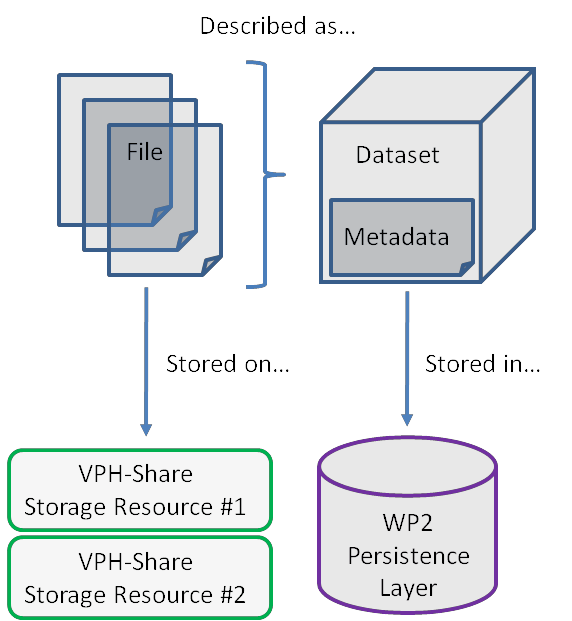
\includegraphics[width=0.5\textwidth]{img/managed-dataset.png}
	\caption{Schematic representation of a~VPH-Share Managed Dataset}
	\label{fig:managed-dataset}
\end{figure}

\noindent
Each managed dataset may consist of an arbitrary number of files(in the simplest case, just 1 file), to which a selection of metadata is appended and stored in WP2 Persistence Layer. Managed datasets map directly to data resource objects described in section 4.4.6, where each dataset consists of one or more DataResource entries. Thus, the description of managed datasets will necessarily include all the metadata associated with data resources, in addition to some DRI-specific metadata. Initially, the DRI managed dataset metadata is expected to consist of the following elements:

\begin{itemize}
\item \textbf{owner} -- reference to VPH-Share user ID of dataset creator,
\item \textbf{list of data items} -- list of data resources ids,
\item \textbf{is managed} -- marker determining whether dataset is under DRI management,
\item \textbf{DRI status} -- dataset's reliability and integrity status,
\item \textbf{date of registration}
\end{itemize}

\noindent
Additionally, each data item will consist of the following attributes:

\begin{itemize}
\item \textbf{owner} -- reference to VPH-Share user ID,
\item \textbf{method of generation} -- uploaded manually, generated by a VPH-Share Atomic Service Instance or registered externally,
\item \textbf{date of registration}
\item \textbf{checksum} -- file's value of a cryptographic hash function calculated upon registration and used to validate integrity and availability of file,
\item \textbf{list of storage resources} -- to which the file is currently deployed (internal reference to WP2 Persistence Layer data storage schema(see section 4.4.6),
\item \textbf{access log} -- as reported by Atmosphere.
\end{itemize}

\noindent
While this schema is expected to cover all the requirements addressed in the Project's Description of Work and in Deliverable D2.1, we foresee that additional metadata can become necessary at later stages in the Project's lifecycle. To this end, the metadata schema will be extensible without the need to clear the contents of the WP2 internal registry. Any updates to the managed dataset schema will be reported and elaborated upon in subsequent WP2 deliverables(i.e. platform prototype descriptions).

\subsubsection{Tagging datasets}
Before automatic verification of managed datasets can take place, it is first necessary to tag specific data as subject for management. It is foreseen that the DRI component will invlove a user interface extension(portlet-based) to enable authorised administrators(possessing a specific role) to tag specific datasets for automatic management(please refer to section 2 for a description of VPH-Share administrator responsibilities). This interaface will display the existing data storage resources and allow creation of new managed datasets consisting of selected files. For each new dataset tagged by administrators, a selection can be supplied automatically by the system - at a minimal level of involvement, the administrator will merely be asked to provide a unique name for a newly created set. As an extension of the user interface, the administrators will also be able to modify and/or purge selected datasets.\\

\noindent
In addition to UI based tagging, the DRI component will also provide API-level access for the same purpose, whenever a VPH-Share application(or workflow) needs to tag specific data as a managed dataset. This option will be provided in the context of useful data generated by applications as opposed to data registered manually by end users. See section 4.5.4 for further details.

\subsubsection{The DRI Runtime Service}
The DRI Runtime is responsible for enforcing Task 2.5 data management policies. It keeps track of managed components and periodically verifies the accessibility and integrity of the managed data. It is expected to operate autonomously(without having to be invoked by administrators) although it will respect the policies defined as part of the managed dataset metadata descriptions and stored in the WP2 persistence layer.\\

\noindent
The DRI Runtime will be implemented as a generic(i.e. non-application-specific) Atomic Service in the WP2 infrastructure. Thus, it can be managed and deployed by Atmosphere tools, just like any other type of Atomic Service. For scalability purposes, multiple instances of DRI Runtime may coexist in the system, integrated into a coherent platform by sharing a common registry(the WP2 persistence layer).\\

\noindent
In line with the Atomic Service specification described in section 3, the DRI Runtime will be deployed into a virtual machine and then registered with Atmosphere mechanisms for automatic management. It is envisioned as a persistent Atomic Service(i.e. once running, it would not be subject to automatic recall, except as requested by system administrators). At the core of the service is an application that periodically polls the WP2 internal registry for lists of managed datasets and then proceeds to verify the following:

\begin{itemize}
\item the availability of each dataset at locations read from the internal registry,
\item the integrity of each dataset(checksum-based validation).
\end{itemize}

\noindent
The DRI Runtime will contact individual storage resources(registered for use in the VPH-Share project) and validate the integrity and availability of the data stored on these resources. Should errors occur, the DRI Runtime will invoke a notification service to issue a warning message to subscribed system administrators(typically, the user defined as the dataset's owner).\\

\noindent
In addition to controlling the availability and integrity of data stored in the Cloud infrastructure, the DRI component will also be able to schedule data replication with Task 2.4 tools, when requested by the administrator or by the Atmosphere application execution components. Again, the same request can be issued manually(via the appropriate Master UI extension) or by invoking an API method of the DRI Runtime. DRI will recognise data storage resources to replicate a dataset to one or more storage resources. This feature may be exploited by Atmosphere to ensure that computations occur in close proximity to data, which is an important prerequisite of maintaining competitive performance of the platform as a whole.

\subsubsection{Persistence schema}
Along with data model of Task 2.4 described in section 4.4.6, managed dataset in section 4.5.1 and DRI Runtime description, the part of metadata schema accessed by the DRI component in presented in Figure \ref{fig:data-model}.\\

\begin{figure}[h!]
	\centering
	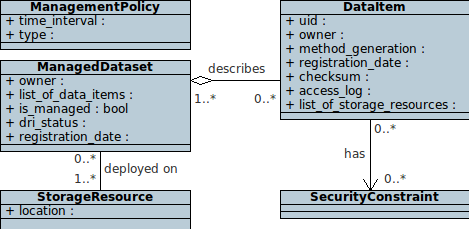
\includegraphics[width=0.8\textwidth]{img/data-model.png}
	\caption{DRI Persistence Schema}
	\label{fig:data-model}
\end{figure}

\noindent
As can be seen above, specific security constraints can be attached to data items, i.e. it cannot be used in public clouds. In DRI component periodic validity checks are of configurable policy via management policy that can be changed by system administrators.\\

\noindent
Again, we foresee that additional metadata can become necessary at later stages in the Project's lifecycle.

\subsubsection{DRI Interfaces}
As hinted upon in the preceding sections, DRI will provide end-user interfaces in the form of a Master UI portlet, as well as an API implemented by the Runtime service, where DRI features may be invoked directly by other VPH-Share intrastructure components.\\

\noindent
The specifics of the DRI portlet will be elaborated upon in the corresponding WP6 deliverable; here we intend to focus on the API, which will provide access to the low-level functionality of DRI and enable it to be configured.\\

\noindent
As DRI exposes a stateless Web Service, all configuration parameters are stored in the Atmosphere Internal Registry. Whenever a configuration change request in invoked the DRI will automatically update policies stored in AIR. In light of this, the DRI API should support the following operations:

\begin{itemize}
\item \textbf{\textit{getStorageResources(): StorageResourceID[]}} -- returns a list of currently registered data storage resource identifiers,
\item \textbf{\textit{getStorageResource(storageResourceID): StorageSiteDescription}} -- returns the information on a specific storage resource, as stored in the Atmosphere Internal Registry in a form of XML document describing the structure of storage resource,
\item \textbf{\textit{registerManagedDataset(DatasetDescription) : datasetID}} -- tags a new dataset for management with Task 2.5 given in the form XML document describing the structure of the dataset, 
\item \textbf{\textit{alterManagedDataset(DatasetID, DatasetDescription) : void}} -- changes the dataset specification stored in the Atmosphere Internal Registry. This action should be used to add or remove files from a managed dataset,
\item \textbf{\textit{removeManagedDataset(DatasetID) : void}} -- excludes the specified dataset from automatic management. This does not delete the data, it merely stops DRI Runtime from polling them,
\item \textbf{\textit{getManagedDataset(DatasetID) : ManagedDatasetDescription}} -- requests information on a specific managed dataset stored in the Atmosphere Internal Registry, returning XML document specyfing the structure of the managed dataset,
\item \textbf{\textit{getOwnerManagedDataset(User) : DatasetID[]}} -- returns a list of user's managed dataset ids,
\item \textbf{\textit{assignDatasetToResource(DatasetID, StorageResourceID) : void}} -- requests DRI to monitor the availability of a specific managed dataset in a specific storage resource. If this dataset is not yet present on the requested storage resource, it will be automatically replicated there with the use of Task 2.4 tools,
\item \textbf{\textit{unassignDatasetFromResource(DatasetID, StorageResourceID) : void}} -- requests DRI to stop monitoring the availability of a specific managed dataset on a specific storage resource. If the dataset is not present on the selected storage resource, this action has no effect,
\item \textbf{\textit{validateManagedDataset(DatasetID) : output}} -- performs asynchronous validation of the specific dataset and produces a document which lists any problems encountered with the dataset's availability on the storage resources to which it bad been assigned,
\item \textbf{\textit{setManagementPolicy(ManagementPolicy) : void}} -- changes monitoring parameters. ManagementPolicy is an XML document specifying the frequency and type of availability checks performed on managed datasets,
\item \textbf{\textit{getManagementPolicy() : ManagementPolicy}} -- retrieves an XML description of the management policy.
\end{itemize}

\begin{figure}[h!]
	\centering
	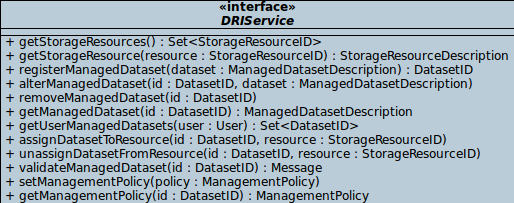
\includegraphics[width=0.8\textwidth]{img/dri-interface.png}
	\caption{DRI Service interface}
	\label{fig:dri-interface}
\end{figure}


\noindent
Each invocation will need to be augmented by the security token which can be intercepted and parsed by the security Policy Enforcement Point residing on the virtual machine on which the DRI Runtime operates. This issue is out of scope of this section, but will be covered in more detail in section 4.6.\\


\subsubsection{DRI architecture}
According to the descriptions and requirements presented in previous sections a DRI component's class diagram can be designed. It is depicted in Figure \ref{fig:dri-service}.\\

\begin{figure}[h!]
	\centering
	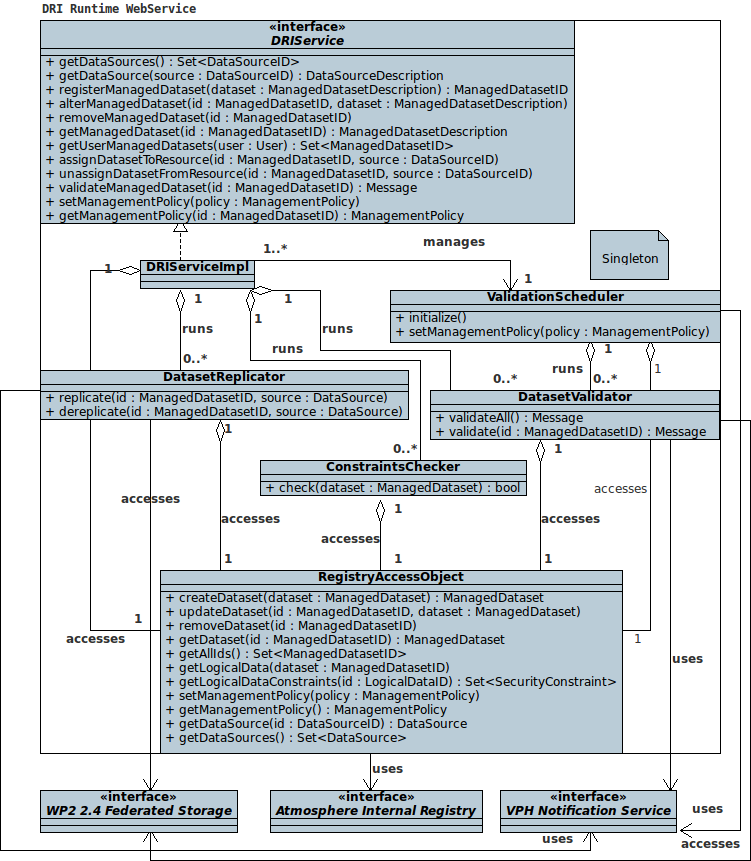
\includegraphics[width=0.8\textwidth]{img/dri-service.png}
	\caption{DRI Runtime class diagram}
	\label{fig:dri-service}
\end{figure}

\noindent
DRI Service interface has already been described(see section 4.5.5).\\

\noindent
Two main tasks performed by DRI Runtime are: validation and replication of managed dataset. DatasetValidator and DataReplicator serve these purposes, respectively. DatasetValidator class encapsulates data reliability and integrity mechanisms exposed by the method \textit{validate()}. Analogously, the DatasetReplicator class represents mechanisms for dataset replication across storage resources through methods \textit{replicate()} and \textit{dereplicate()}. Both classes access WP2 Federated Storage for data access and VPH Notification Service for error reporting. Concrete DRIService implementation runs these two to perform crucial service tasks. \\

\noindent
As mentioned in section 4.5.4, specific data items can have security constraints, which should be checked before performing update operations on managed datasets. In our design, separate ConstraintsChecker class was designated for this task exposing \textit{check()} method.\\

\noindent
RegistryAccessObject enables other classes of DRI component access to persistence data stored in Atmosphere Internal Registry. Methods exposed are CRUD-like(create, read, update, delete) fashion. Additionally, such persistence access layer release other classes from possible raw AIR access complexities.\\

\noindent
Periodic data reliability and integrity checks will be run by ValidationScheduler in configurable time periods. Singleton design pattern should perfectly meet its design needs.\\

\noindent
DRI Runtime is completely stateless WebService. All its data is saved and retrieved from Atmosphere Internal Registry through RegistryAccessObject.

\subsubsection{Validation \& replication mechanisms}
DRI Runtime class diagram depicted in previous section can be well utilized to describe validation and replication mechanisms flows in detail.\\

\noindent
The following two sequence diagrams in Figure \ref{fig:validation-diagram} and \ref{fig:replication-diagram}.\\

\begin{figure}[h!]
	\centering
	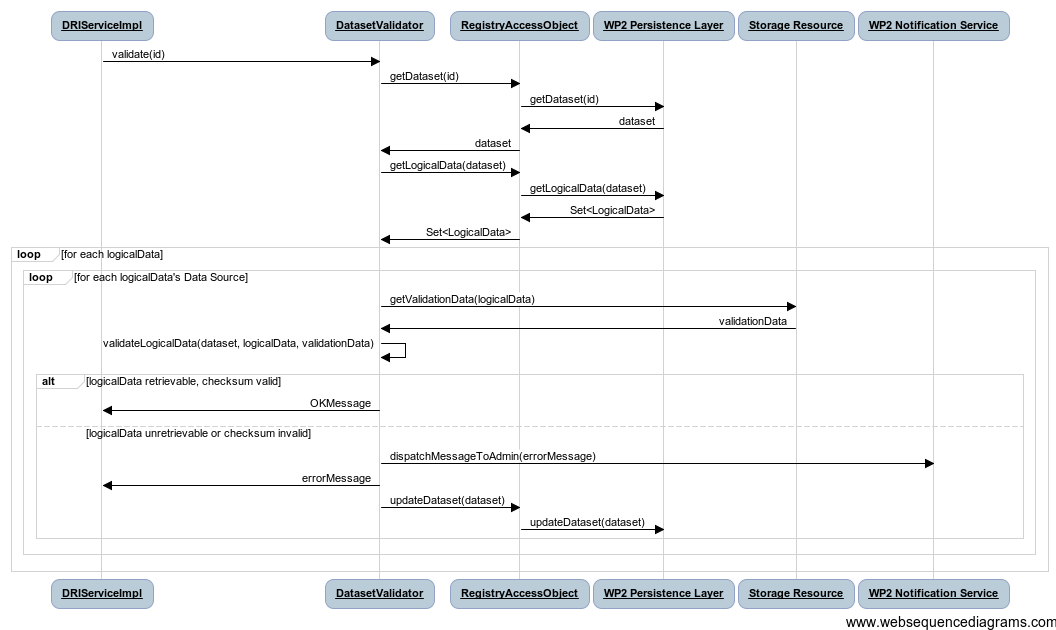
\includegraphics[width=1.0\textwidth]{img/validation-diagram.png}
	\caption{DRI validate() call sequence diagram}
	\label{fig:validation-diagram}
\end{figure}

\begin{figure}[h!]
	\centering
	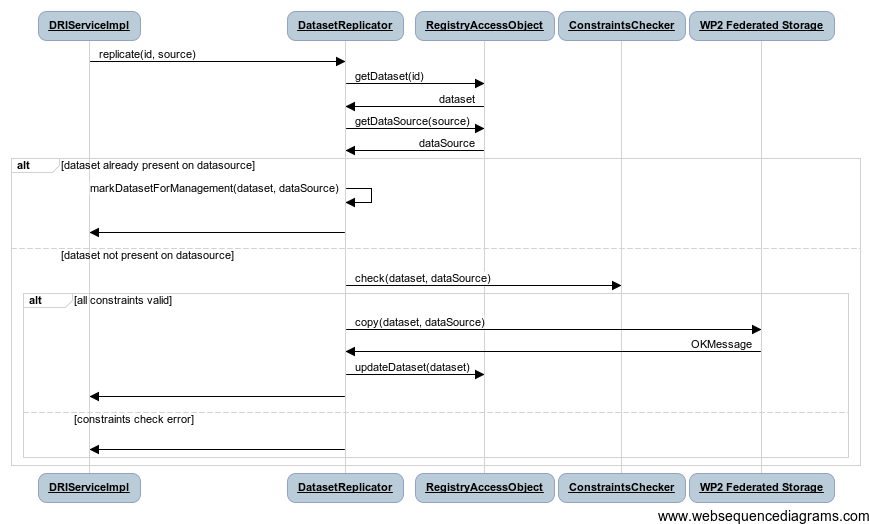
\includegraphics[width=1.0\textwidth]{img/replication-diagram.png}
	\caption{DRI assignDatasetToResource() call sequence diagram}
	\label{fig:replication-diagram}
\end{figure}

\noindent
Upon \textit{validate()} call, the DRIService will invoke DatasetValidator object to apply data reliability and integrity check on the specified dataset. Subsequently, the DatasetValidator will retrieve specified managed dataset and data items which it is describing using RegistryAccessObject. Validation occurs against specific resources storing data items replicas by retrieving validation data, calculating checksum and comparing it with the one stored in data item entry. If all dataset's data items appear retievable and valid, the DatasetValidator returns OK message. Otherwise it sends error message to the WP2 Notification Service and updates dataset status to \textit{invalid}. Dataset's integrity check breaks at first data item error.\\

\noindent
Upon \textit{assignDatasetToResource()} call, the DRIService will invoke DatasetReplicator object to replicate specified dataset to user-chosen storage. After retrieving specified managed dataset and storage resource objects from RegistryAccessObject the DataReplicator will check whether the dataset is already present on specified storage resource. If yes, then only mark for management will occur. Otherwise, the security constraints must be checked, if valid, then replication takes place using WP2 Federated Storage mechanisms and dataset metadata update.

\subsubsection{Scalability issues}
In order to cope with a significant number of big datasets, multiple instances of DRI Runtime can be deployed. As long as DRIService stays stateless WebService there are no big inconsistency threats. ValidationScheduler will be implemented in Master-Slave pattern to load balance the validation's performance cost.

\subsubsection{Implementation Technologies}
The DRI Runtime will be developed as a standalone application set up on a virtual machine obtained from Atmosphere management services(Task 2.1) and registered as a persistent Atomic Service. Following launch(which will occur automatically whenever an instance of the Runtime is deployed), the application will enter a cycle(of configurable duration) where at fixed time intervals it will contact the WP2 registry and subsequently validate managed datasets with the use of Task 2.4 access tools.\\

\noindent
The application will be developed in Java. An application of the Runtime will be deployed to an application server and expose a RESTful Web Service API(Jersey implementation), which will provide the backend functionality of the DRI component. The Java framework used will be Spring. For validation scheduling Quartz Scheduler will be utilized. The service will be secured with the authenticity tokens and will contact the Task 2.6 Policy Decision Point(see section 4.6 for details) to guard against unauthorised access. Console access to the virtual machine on which DRI components reside will be limited to WP2 developers and/or system administrators.\\

\noindent
The Atmosphere Internal Registry will be the persistence layer used to store DRI metadata and descriptions of managed datasets. A discussion of the technologies used in its implementation can be found in section 4.1.\\

\noindent
User interace extensions will be implemented using a Portlet-2.0 compliant interface, in Java; however the decision on which specific portal platform to adopt for the VPH-Share Master Interface rests with WP6. The issue will be addressed in D6.2, which is due by Month 9 of the Project. Regardless, it is expected that the portlet solution developed in Task 2.5 will remain compatible with the Mater Interface by way of compliance with the JSR-286 standard(52).

\end{document}
